%        File: pattern_report2014.tex
%     Created: Thu Jan 22 03:00 AM 2015 J
% Last Change: Thu Jan 22 03:00 AM 2015 J
%
\documentclass[10pt,a4paper]{jarticle}

%%%%%%%%%%%%%%%%%%%%%
% to input Japanese %
%%%%%%%%%%%%%%%%%%%%%
\usepackage[japanese]{babel}

%%%%%%%%%%%
% unknown %
%%%%%%%%%%%
\usepackage{ascmac}

%%%%%%%%%%%%%%%%%%%%%%%%%%
% to be standard a4paper %
%%%%%%%%%%%%%%%%%%%%%%%%%%
\usepackage{geometry}
\geometry{left=20mm, right=20mm, top=20mm, bottom=40mm}

%%%%%%%%%%%%%%%%%%%%%
% to insert figures %
%%%%%%%%%%%%%%%%%%%%%
\usepackage[dvipdfmx]{graphicx}

%%%%%%%%%%%%%%%%%%%%%%%%%%
% to insert source codes %
%%%%%%%%%%%%%%%%%%%%%%%%%%
% \usepackage{listings, jlisting}
% \renewcommand{\lstlistingname}{list}
% \lstset{language=C,
%   basicstyle=\ttfamily\scriptsize,
%   commentstyle=\textit,
%   classoffset=1,
%   keywordstyle=\bfseries,
%   frame=tRBl,
%   framesep=5pt,
%   showstringspaces=false,
%   numbers=left,
%   stepnumber=1,
%   numberstyle=\tiny,
%   tabsize=2
% }

%%%%%%%%%%%%%%%%%%
% title & author %
%%%%%%%%%%%%%%%%%%
\title{パターン情報学 プログラミングレポート課題}
\author{03-140299 東京大学機械情報工学科 3年 和田健太郎}

%%%%%%%%%%%%%%%%%%
% begin document %
%%%%%%%%%%%%%%%%%%
\begin{document}
\maketitle

\section{課題1}\label{section:kadai1}
\begin{itembox}{課題1}
2 クラス($\omega$1,$\omega$2)の識別問題を考える.データは 2 次元とする.配布するデータセットの説明を以下に示す.

\begin{itemize}
  \item Train1.txt,Train2.txt:$\omega$1,$\omega$2 に属する訓練データ集合.各データ数 50.
  \item Test1.txt,Test2.txt: $\omega$1,$\omega$2 に属するテストデータ集合.各データ数 20.
\end{itemize}

2 クラスで,2 次元のデータに対するウィドロー・ホフのアルゴリズムを実装し,訓練データから分離超平面を
学習せよ.また,テストデータの識別率(全テストデータ数に対する正しく識別されたテストデータ数の比率)を
求めよ.さらに,訓練データ,テストデータ,学習された識別面を図示せよ.
\end{itembox}
ウィドロー・ホフのアルゴリズムを初期の重みはランダムとし, 
指定した回数だけ繰り返し重みの更新を行うように実装した. 

2次元の訓練データ100件を用いて識別器の学習を行い, 40件のテストデータで
性能を測定したところ, 0.875という結果が出た. 

また, 訓練データ, テストデータのそれぞれ2クラスと識別面を図示したものが
図\ref{fig:kadai1}である. 

\begin{figure}[htbp]
  \centering
  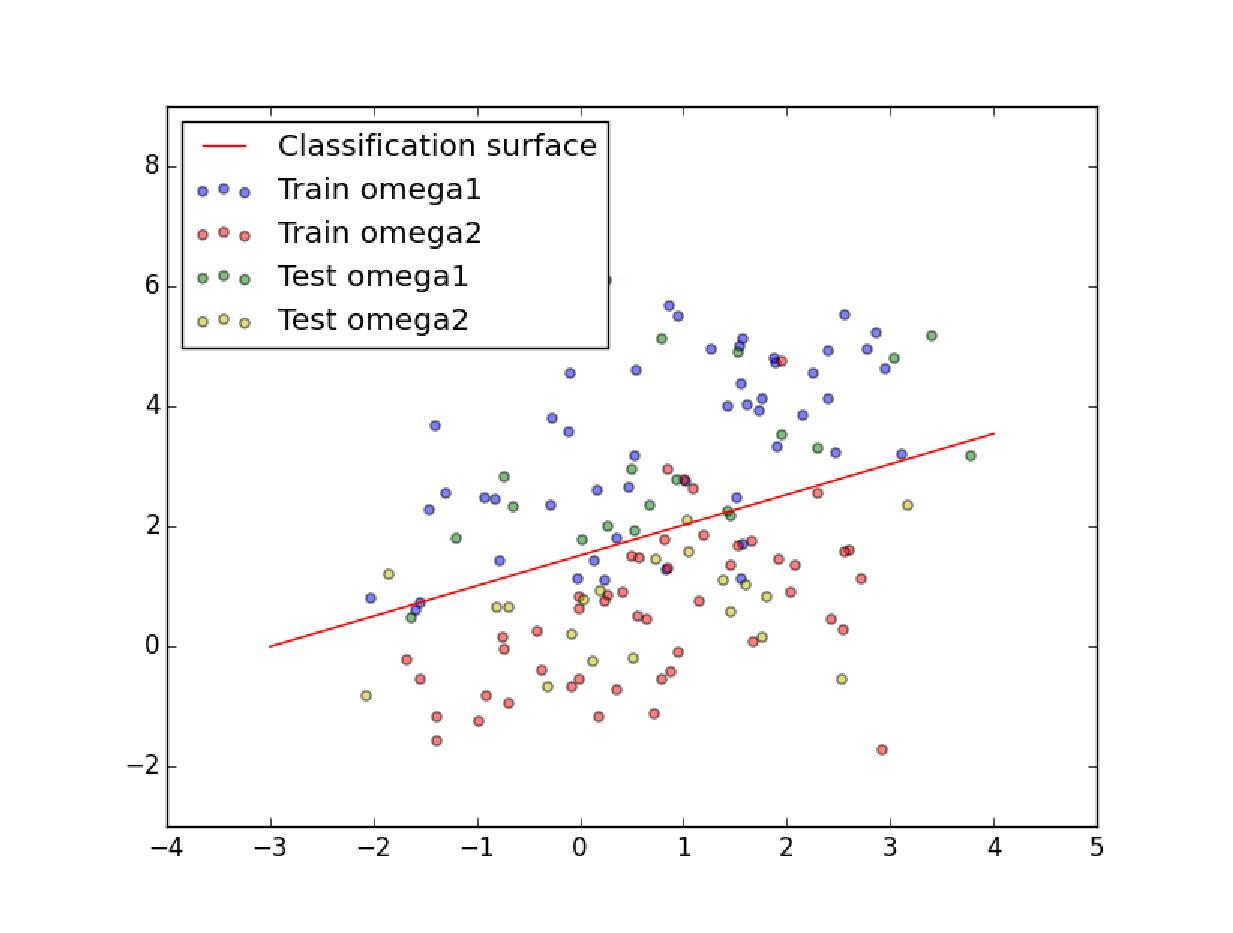
\includegraphics[width=0.7\textwidth]{./assets/kadai1_plot_20150122_031552.eps}
  \caption{データおよび識別面}
  \label{fig:kadai1}
\end{figure}


\section{課題2}\label{section:kadai2}
\begin{itembox}{課題2}
  擬似逆行列を計算するプログラムを書き,課題 1 と同じ訓練データから分離超平面を学習せよ.
  また,テストデータの識別率を求めよ.
  クラスラベルについて,$\omega$1 に属するものを 1,$\omega$2 に属するものを-1 などとせよ.さらに,学習された識別面を課題 1 と同じ図に示せ.
\end{itembox}

擬似逆行列を数値計算ライブラリであるnumpyを利用して実装した. 

\begin{eqnarray*}
  A^{+} = (A^{T} \cdot A)^{-1} \cdot A^{T}
\end{eqnarray*}

擬似逆行列を用いて訓練データに関して重みを計算し, 
テストデータによって識別性能を測定したところ,~\ref{section:kadai1} と
同様に0.875という結果だった. 

訓練データ, テストデータおよび識別面を図示したものが
図\ref{fig:kadai2}で, 識別面の位置をウィドロー・ホフのアルゴリズム
によるものと比べてみると, ほぼ同じ位置にあることがわかる. 

\begin{figure}[htbp]
  \centering
  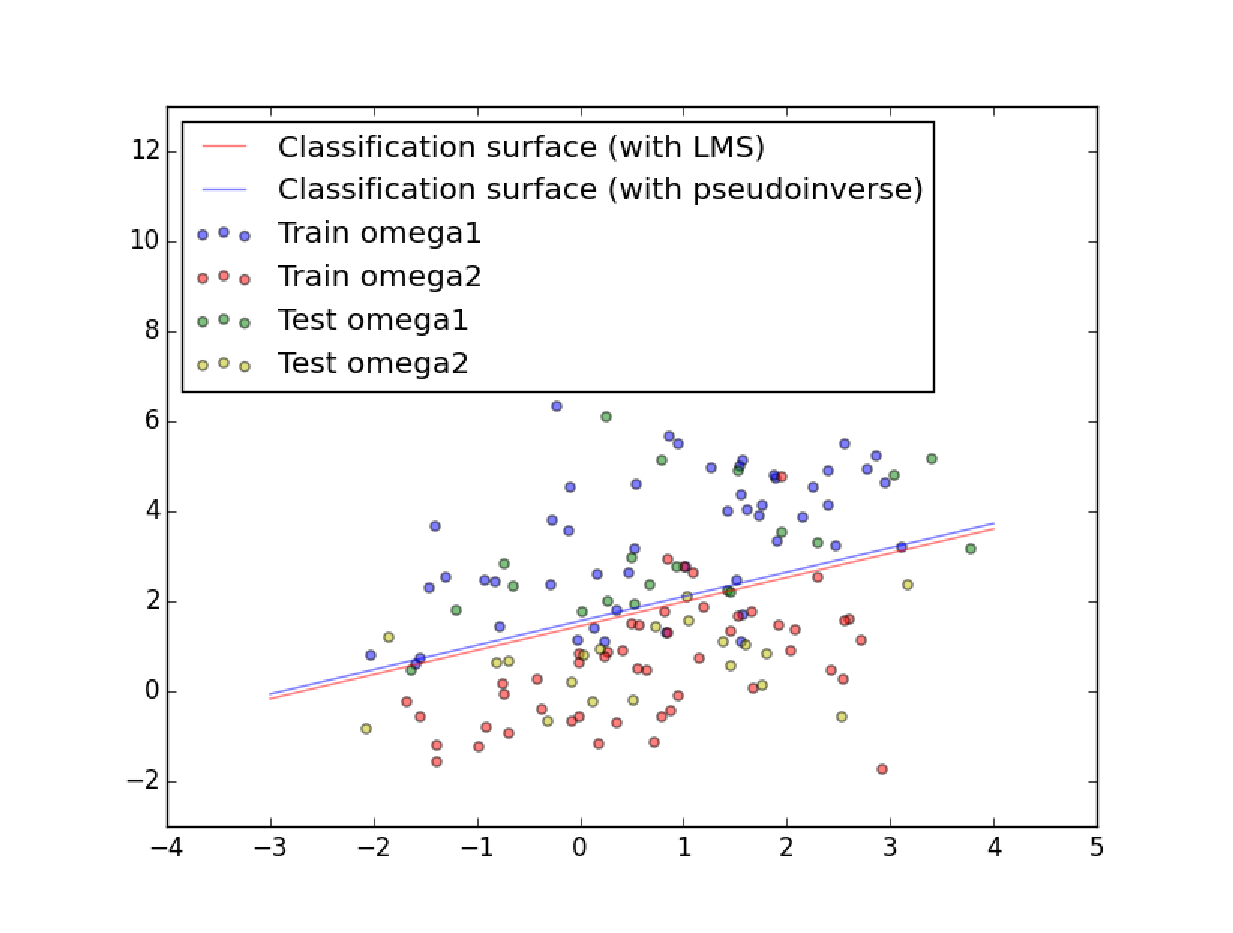
\includegraphics[width=0.7\textwidth]{./assets/kadai2_plot_20150122_031556.eps}
  \caption{データおよび識別面}
  \label{fig:kadai2}
\end{figure}


\section{課題3}
\begin{itembox}{課題3}
  本課題も課題 1 と同じデータセットを利用する.
  \begin{enumerate}
    \item テストデータの集合を k 近傍法 (kNN) を用いて識別することを考える. 訓練データに対して一つ抜き出し, (LOO: leave-one-out) 法により k の値を 1 から 10 まで変化させ,最適な k の値を求めよ.また,横軸に k, 縦軸に識別率としてグラフを作成せよ.
    \item LOO により得られた k の値を用いてテストデータを識別せよ.そして,識別率を求めよ.
  \end{enumerate}
\end{itembox}
訓練データに対してLOOにより識別を行い, kの値を1から10まで変化させて識別率を測定した. 
その関係を示したのが図\ref{fig:kadai3}である. 
\begin{figure}[htbp]
  \centering
  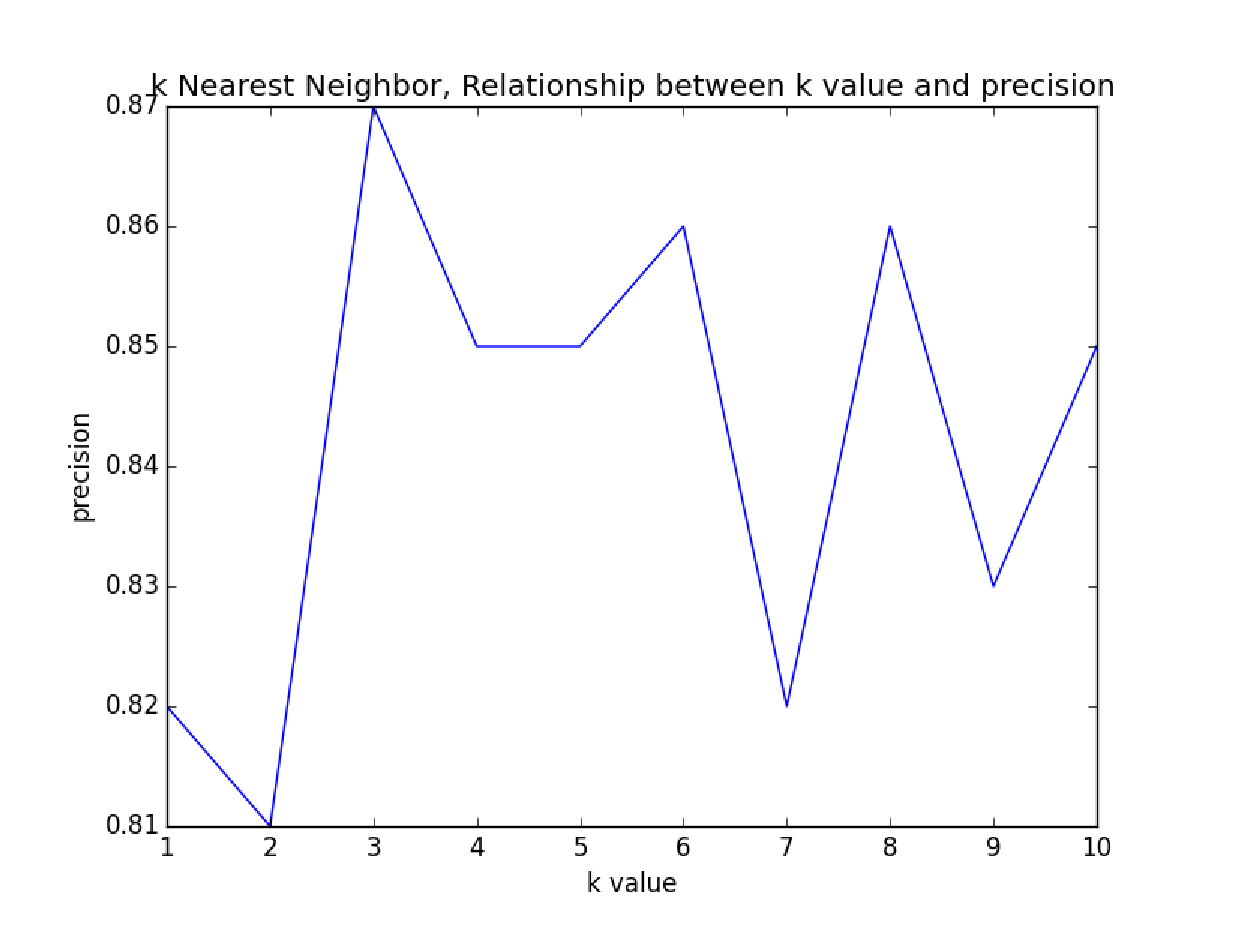
\includegraphics[width=0.4\textwidth]{./assets/kadai3_various_kvalue_20150121_231435.eps}
  \caption{k値とLOO法によるkNNの識別率の関係}
  \label{fig:kadai3}
\end{figure}
図\ref{fig:kadai3}より,kが3の時に最も識別性能が高くなっていることが
わかる.


\section{課題4}
\begin{itembox}{課題4}
  表にあるデータを利用する.また潜在的な確率密度分布は正規分布であるとする.P($\omega$i)=1/3 とする.表にあ
  げた各クラスのデータセットは omega1.txt,omega2.txt,omega3.txt である.このとき次の問いに答えよ.

  \begin{enumerate}
    \item テスト点:$(1, 2, 1)^T$, $(5, 3, 2)^T$, $(0, 0, 0)^T$, $(1, 0, 0)^T$ と各クラスの平均との間のマハラノビス距離を求めよ.
    \item これらの点を識別せよ.
    \item 次に P($\omega_1$)=0.8 かつ P($\omega_2$) = P($\omega_3$)=0.1 と仮定し,テスト点をもう一度識別せよ
  \end{enumerate}
\end{itembox}
テスト点:$(1, 2, 1)^T$, $(5, 3, 2)^T$, $(0, 0, 0)^T$, $(1, 0, 0)^T$
に関して, 各クラス集合の平均とのマハラノビス距離

\begin{eqnarray}
  M_{D}(x) = \sqrt{(x - \mu_{i})^T \sum (x - \mu_i)}
\end{eqnarray}

を表\ref{tbl:mahalanobis}に計算した. 

\begin{table}[htbp]
  \begin{small}
    \begin{tabular}{cccc}
      sample points & $\omega_1$ & $\omega_2$ & $\omega_3$ \\
      $(1, 2, 1)^T$ & 21.275575 & 15.5762194 & 9.85157479 \\
      $(5, 3, 2)^T$ & 39.1226698 & 37.4144013 & 9.82164589 \\
      $(0, 0, 0)^T$ & 9.175011 & 4.78336417 & 23.4702917 \\
      $(1, 0, 0)^T$ & 12.0187365 & 9.85778568 & 20.7996021
    \end{tabular}
    \caption{テスト点の各クラス集合の平均とのマハラノビス距離}
    \label{tbl:mahalanobis}
  \end{small}
\end{table}

確率的生成モデルを用いて, これらのテスト点を識別したところ, 
表\ref{tbl:prob-discrimination-1}に示す識別結果となった. ($P(\omega_i)$ = 1/3)

$P(\omega_1)=0.8$, $P(\omega_2)=P(\omega_3)=0.1$として識別を行ったところ
表\ref{tbl:prob-discrimination-2}に示す識別結果となり, 
表\ref{tbl:prob-discrimination-1}と同じ結果となった. 

\begin{table}[htbp]
  \begin{tabular}{cccc}
    % test point 1 & test point 2 & test point 3 & test point 4 \\
    $(1, 2, 1)^T$ & $(5, 3, 2)^T$ & $(0, 0, 0)^T$ & $(1, 0, 0)^T$ \\
    $\omega_2$ & $\omega_2$ & $\omega_1$ & $\omega_1$
  \end{tabular}
  \caption{$P{\omega_i}=1/3$での識別結果}
  \label{tbl:prob-discrimination-1}
\end{table}

\begin{table}[htbp]
  \begin{tabular}{cccc}
    % test point 1 & test point 2 & test point 3 & test point 4 \\
    $(1, 2, 1)^T$ & $(5, 3, 2)^T$ & $(0, 0, 0)^T$ & $(1, 0, 0)^T$ \\
    $\omega_2$ & $\omega_2$ & $\omega_1$ & $\omega_1$
  \end{tabular}
  \caption{$P{\omega_1}=0.8$, $P{\omega_2}=P{\omega_3}=0.1$ での識別結果}
  \label{tbl:prob-discrimination-2}
\end{table}


\section{チャレンジ課題1}\label{section:challenge1}
\begin{itembox}{チャレンジ課題1}
  主成分分析,多クラスフィッシャー判別分析を実装せよ.
  また,3 クラス,4 次元の iris データセット iris.txt に
  主成分分析とフィッシャー判別分析をそれぞれ適応して 1 次元に
  次元削減し図示せよ.
  次元削減後のクラス間デー タの分離の違いを確認せよ.
  なお iris データセットの各行はデータのインデックス,
  第 5 列はクラス番号(1,2, 3 クラス)を示している.
  各クラス 50 サンプル合計 150 サンプルとなる.
\end{itembox}

主成分分析とフィッシャー線形判別による特徴空間の
変換結果を~\ref{fig:challenge1}に示す.

PCAに比べFisherLDAではクラス1とクラス2,3とのクラス間分散が大きくなり,
クラス3のクラス内分散が小さくなっていることがわかる.
また,クラス2,3の重なりもFisherLDAの方が小さくなっている.


\begin{figure}[htbp]
  \centering
  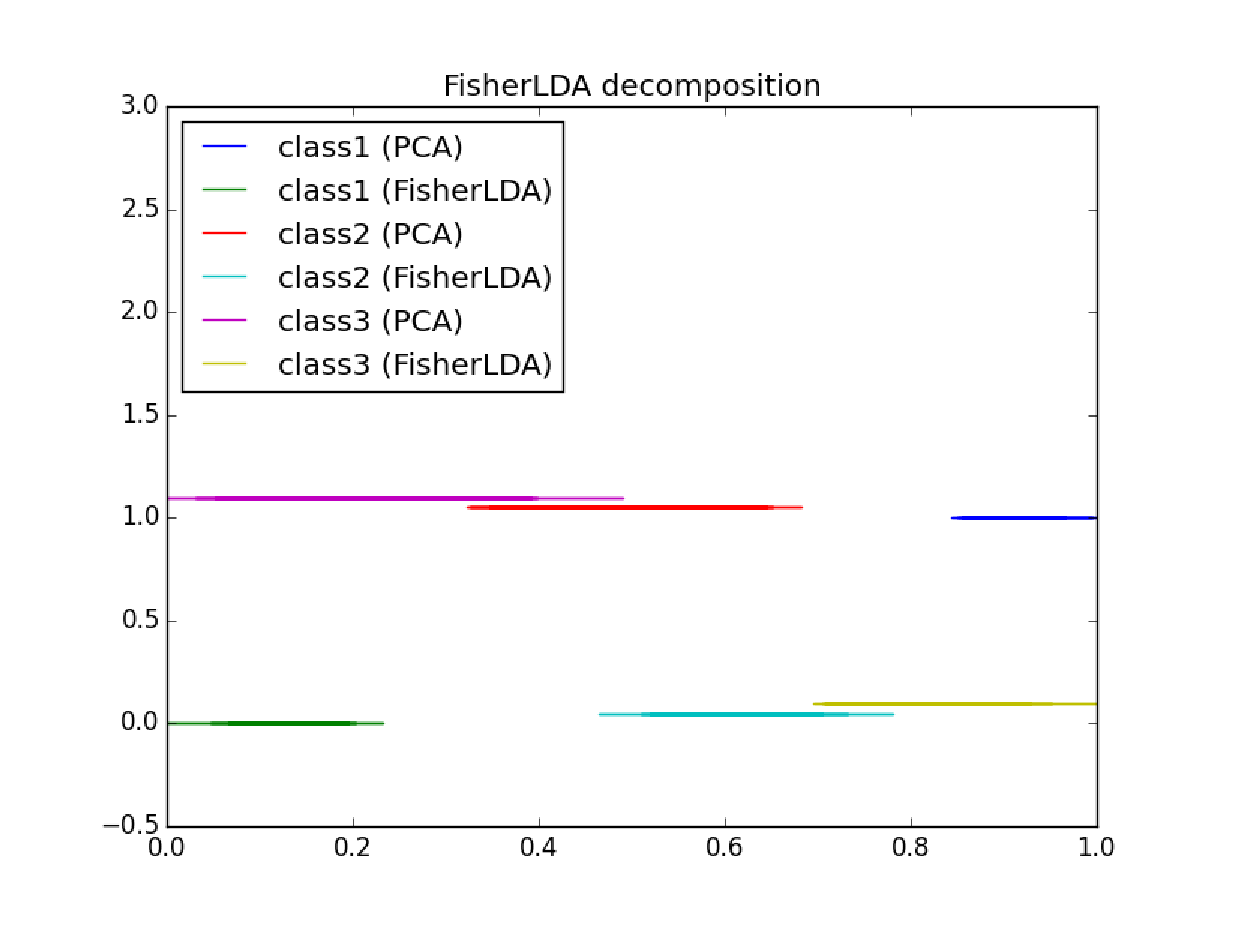
\includegraphics[width=0.8\textwidth]{./assets/challenge1_plot_20150210_050430.eps}
  \caption{PCAとFisherLDAによる特徴空間の変換(データ:iris.txt)}
  \label{fig:challenge1}
\end{figure}
\section{チャレンジ課題2}\label{section:challenge2}
\begin{itembox}{チャレンジ課題2}
  ロジスティック回帰を実装し,
  課題1のデータに適用してテストデータの識別率を求めよ.
\end{itembox}

\begin{figure}[htbp]
  \centering
  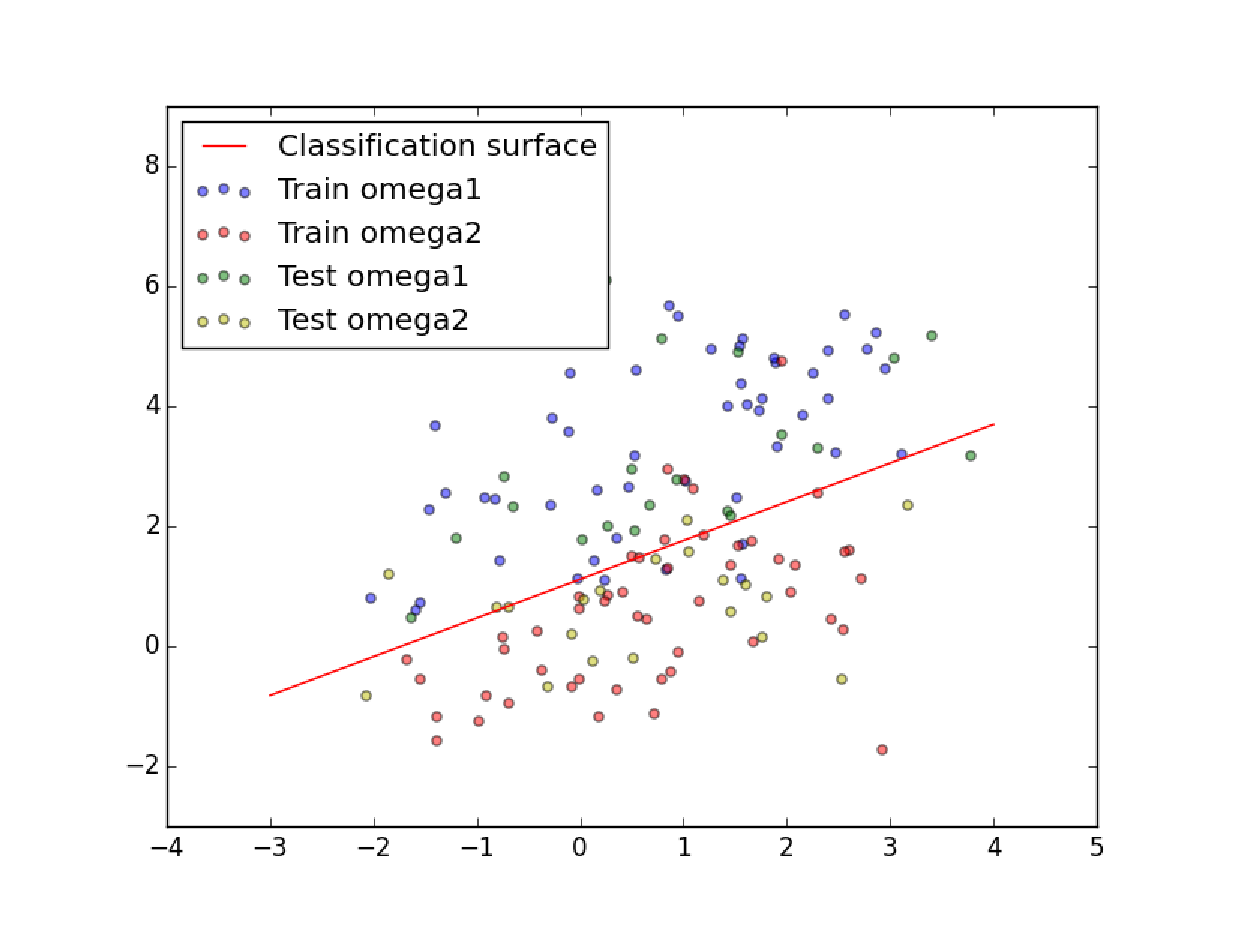
\includegraphics[width=0.8\textwidth]{./assets/challenge2_plot_20150212_000710.eps}
  \caption{ロジスティック回帰による識別}
  \label{fig:challenge2}
\end{figure}


%%%%%%%%%%%%%%%%%%%%%%%%%%
% to insert bibliography %
%%%%%%%%%%%%%%%%%%%%%%%%%%
% \begin{thebibliography}{9}
%   \bibitem{inv1} Samuel R.Buss,"Introduction to Inverse Kinematics with Jacobian Transpose,Pseudoinverse and Damped Least Squares methods"
% \end{thebibliography}

%%%%%%%%%%%%%%%%
% end document %
%%%%%%%%%%%%%%%%
\end{document}

